% !TEX TS-program = pdflatex
% !TEX encoding = UTF-8 Unicode

\documentclass[10pt]{report}
	% set document class
	% default font size is 10pt

\usepackage[utf8]{inputenc} 
	% set input encoding (not needed with XeLaTeX)

\usepackage{cite}
\usepackage{url}

%%% PAGE DIMENSIONS
\usepackage{geometry} % to change the page dimensions
\geometry{a4paper}
% or letterpaper (US) or a5paper or....

\usepackage{graphicx}
	% support for the \includegraphics command and options

\usepackage[parfill]{parskip} % Activate to begin paragraphs with an empty line rather than an indent

%%% PACKAGES
\usepackage{booktabs} % for much better looking tables
\usepackage{array} % for better arrays (eg matrices) in maths
\usepackage{paralist} % very flexible & customisable lists (eg. enumerate/itemize, etc.)
\usepackage{verbatim} % adds environment for commenting out blocks of text & for better verbatim
\usepackage{subfig} % make it possible to include more than one captioned figure/table in a single float
% These packages are all incorporated in the memoir class to one degree or another...

\usepackage{calc}
\usepackage{enumitem}
\usepackage{varioref} % gives us \vref
\usepackage{rotfloat} % allows floats to be rotated

\usepackage{bytefield}

\usepackage{dirtree} % for makin' directory trees (see Deriverables section)

\usepackage{float}
\newfloat{listing}{htbp}{lol}[chapter]
\floatname{listing}{Listing}

\usepackage{pgf}
\usepackage{tikz} % we use this for state machine drawings and stuff
\usetikzlibrary{arrows,automata}

%%% HEADERS & FOOTERS
\usepackage{fancyhdr} % This should be set AFTER setting up the page geometry
\pagestyle{fancy} % options: empty , plain , fancy
\renewcommand{\headrulewidth}{0pt} % customise the layout...
\lhead{}\chead{}\rhead{Assignment \#1, TDT4255 Computer Design}
\lfoot{}\cfoot{\thepage}\rfoot{}

%%% SECTION TITLE APPEARANCE
\usepackage{sectsty}
%\allsectionsfont{\sffamily\mdseries\upshape} % (See the fntguide.pdf for font help)

%%% ToC (table of contents) APPEARANCE
\usepackage[nottoc,notlof,notlot]{tocbibind} % Put the bibliography in the ToC
\usepackage[titles,subfigure]{tocloft} % Alter the style of the Table of Contents
\renewcommand{\cftsecfont}{\rmfamily\mdseries\upshape}
\renewcommand{\cftsecpagefont}{\rmfamily\mdseries\upshape} % No bold!

\newcommand{\subsubsubsection}{\paragraph}

\newcommand\todo[1]{\textcolor{red}{TODO: #1}}
\newcommand\cn{\textcolor{red}{[citation needed]}}


\title{Report for Assignment \#2 \\
TDT4255 Computer Design, NTNU}
\author{Sigve Sebastian Farstad \and
		Rune Holmgren \and
		Odd Magnus Trondrud}

%\date{} % Activate to display a given date or no date (if empty),
         % otherwise the current date is printed 

\begin{document}

\maketitle

\pagenumbering{roman}

\begin{abstract}
	% quick and dirty hack to change the margins
\begin{quote}
\begin{quote}
This report presents a solution to assignment \#2 of TDT4255 Computer Design at the Norwegian University of Technology and Science, autumn 2013.
The assignment was to implement an optimized pipelined processor with a simple MIPS-inspired 5-stage pipeline design, and to program it onto an FPGA.
The solution processor presented in this report fulfils all the requirements given by the assignment, and is delivered together with a fully-featured assembler written in Python.
\end{quote}
\end{quote}

\end{abstract}

\tableofcontents

\listoffigures

\listoftables

\listof{listing}{List of Listings}

\chapter{Introduction}

\pagenumbering{arabic}

	This report presents a solution to ``Assignment \#1 - Simple Multi-cycle MIPS Processor'' of the autumn 2013 course TDT4255 at NTNU.

\section{Assignment}

A summery of the assignment can be found in section 4.1 of the compendium~\cite[p.114]{compendium}, and is reproduced below for convenience:

\begin{quote}
``In this assignment, you will design a simple multi-cycle MIPS processor in VHDL and synthesize your design by following the procedure described in Chapter 2~\cite[of the compendium]{compendium}.
You will also verify the behaviour of the implemented MIPS processor using the ModelSim simulator.
Once your design is verified, you will integrate the MIPS processor into a MicroBlaze-based embedded system as a peripheral core, implement the embedded system design in FPGA\footnote{It was assumed that the assignment author means ``VHDL'' here} and the designed processor in an FPGA.''
\end{quote}

\subsection{Requirements}

The assignment's main requirement is to design a ``simple multi-cycle MIPS architecture''~\cite[p.114]{compendium}. It must be based on the suggested MIPS-like architecture presented in Figure 4.1~\cite[p.115]{compendium} in the course compendium.

Minimally, the instructions from a given set of instruction classes have to be implemented. 
Examination of the list yielded 10 instructions that were deemed a part of the minimum requirement.
These are listed in Table \vref{table:required-instructions}.

\begin{table}
    \begin{center}
        \begin{tabular}{r|l}
            \texttt{ADD} & Add \\
            \texttt{AND} & And \\
            \texttt{BEQ} & Branch if equal \\
            \texttt{J} & Jump \\
            \texttt{LDI}/\texttt{LLI} & Load (lower) immediate \\
            \texttt{LW} & Load word \\
            \texttt{OR} & Or \\
            \texttt{SLT} & Set less than \\
            \texttt{SUB} & Subtract \\
            \texttt{SW} & Store word \\
            \hline
        \end{tabular}
        \smallskip
        \smallskip
        \caption{Required instructions.}
        \label{table:required-instructions}
    \end{center}
\end{table}

Note: the assignment text required the ``\texttt{LDI} (Load Upper Immediate)''\footnote{Verbatim from \cite[p.114]{compendium}} instruction to be implemented.
However in MIPS, \texttt{LDI} is not an instruction.
The closest match in MIPS is the instruction called \texttt{LUI} (Load Upper Immedate).
This instruction loads an immediate, but also shifts it to put it in the upper half of the destination register.
As LUI does not do exactly what LDI would have done, a new instruction \texttt{LLI} (Load Lower Immediate), takes \texttt{LDI}'s place in the instruction requirements table.

Implementing more instructions than the aformentioned is optional.
The instruction set implemented by the solution processor is detailed in section \vref{sec:instruction-set}.

Once the processor is designed, it must also be verified in a simulation environment as well as in a hardware platform.

\section{Goals}

For this assignment, a set of solution goals were decided upon that should be met in addition the the minimal requirements given in the assignment.
All decisions in the process of completing the assignment were made to further the goals in this section.
The three solution goals are presented here in order of descending importance.

\subsection{Industry Standard Best Practices}

The first goal is that, to the extent that is is practically possible, the solution should conform to the current industry standards in aspects such as implementation style, tooling, best practices and so on.
This goal was chosen because the industry has many, many years of combined experience in the field, and using its accumulated knowledge and wisdom for what it is worth can help increase solution stability, ease of development, and avoiding common pitfalls and gotchas.

\subsection{A Large and Diverse Instruction Set}

The second solution goal is that the solution processor should support as much of the MIPS I instruction set as possible.
It should ideally be functionally equivalent to other MIPS I processors.
The reasoning behind this is that the closer the solution processor resembles a regular MIPS processor, the easier it is to employ existing tools, made for other MIPS processors, with the solution processor.
This allows for things like an existing MIPS-supporting C compiler to compile regular C code to run on the solution processor.

\subsection{Performance}

The third and least prioritized solution goal is that the processor should not be slow.
That means that when an architectural or implementation desicion must be made, the choice with a more processor performant outcome should be chosen, as long as it does not conflict with the other design goals.
This means that it is ok to sacrifice processor performance if doing so results in better conformance to industry standards or support for more instructions.



\chapter{Solution Description}
	The processor presented as a solution for assignment 1 in this report is a simple 32-bit MIPS-inspired multi-cycle processor described in VHDL.
It was attempted programmed onto a Xilinx Spartan-6 LX25 FPGA.

\section{Solution Architecture}

The processor architecture is a MIPS-inspired pipelined architecture with five stages.
The five stages are called Instruction Fetch, Instruction Decode, Execution, Memory and Write Back.
Each stage is separated by pipeline registers that hold the relevant data for the different stages between clock cycles.
Since the the CPU is pipelined, it can achieve much higher performance than the simple multi-cycle processor architecture designed in the previous assignment\cite{assignment-1}.
For ideal execution, every component of the processor is in use in every cycle, giving a high utilization of resources.
Paradoxically, even though pipelined processor designs can be much more performant than simple multi-cycle processor designs, they are not necessarily more complex.
This is because there is no longer need for a massive state machine in the control unit in the pipeline processor, as there would be in a multi-cycle processor control unit.

Not everything is better with a pipelined design, however.
With a pipelined design, the processor is vulnerable to data hazards and control hazards.
A hazard, in processor design terminology, is a situation where a planned execution in a processor cannot be performed because it is dependant on the outcome of a previous execution which has not yet completed.
This is made possible because of the introduction of instruction-level parallelism.
The solution processor presented in this report resolves hazards by using a combination of data forwarding and stalling.
One type of hazard, the use-after-load\cn hazard, where an instruction relies on the data from a memory load in the instruction immediately preceding it, is not handled by the processor.
Trying to execute an instruction which uses the result from a load immediately after the load instruction results in undefined behaviour.
Instead of handling this in hardware, the bundled solution assembler solves this issue by instruction reordering, or simply inserting nops where needed.
This is done to remove complexity from the processor core, which in turn increases processor performance, which is aligned with the performance goal from section \vref{subsection:performance}.

The processor architecture is modeled after the Harvard Architecture design, which means that it has separate instruction and data memory.
This, in addition to being a security boon, makes for a more performant design, as the instruction memory and data can be accessed independently.
This is aligned with the performance design goal from \vref{subsection:performance}.

Having separate memories for data and instructions also removes the need for a central memory access arbitrage unit, which increases the simplicity of the design in accordance to the design goal in section\vref{subsection:simplicity}.

The processor architecture can bee seen illustrated in figure \vref{figure:architecture}.
The tall orange bars are the pipeline registers.
The blue lines are control signals.

\begin{figure}[H]
    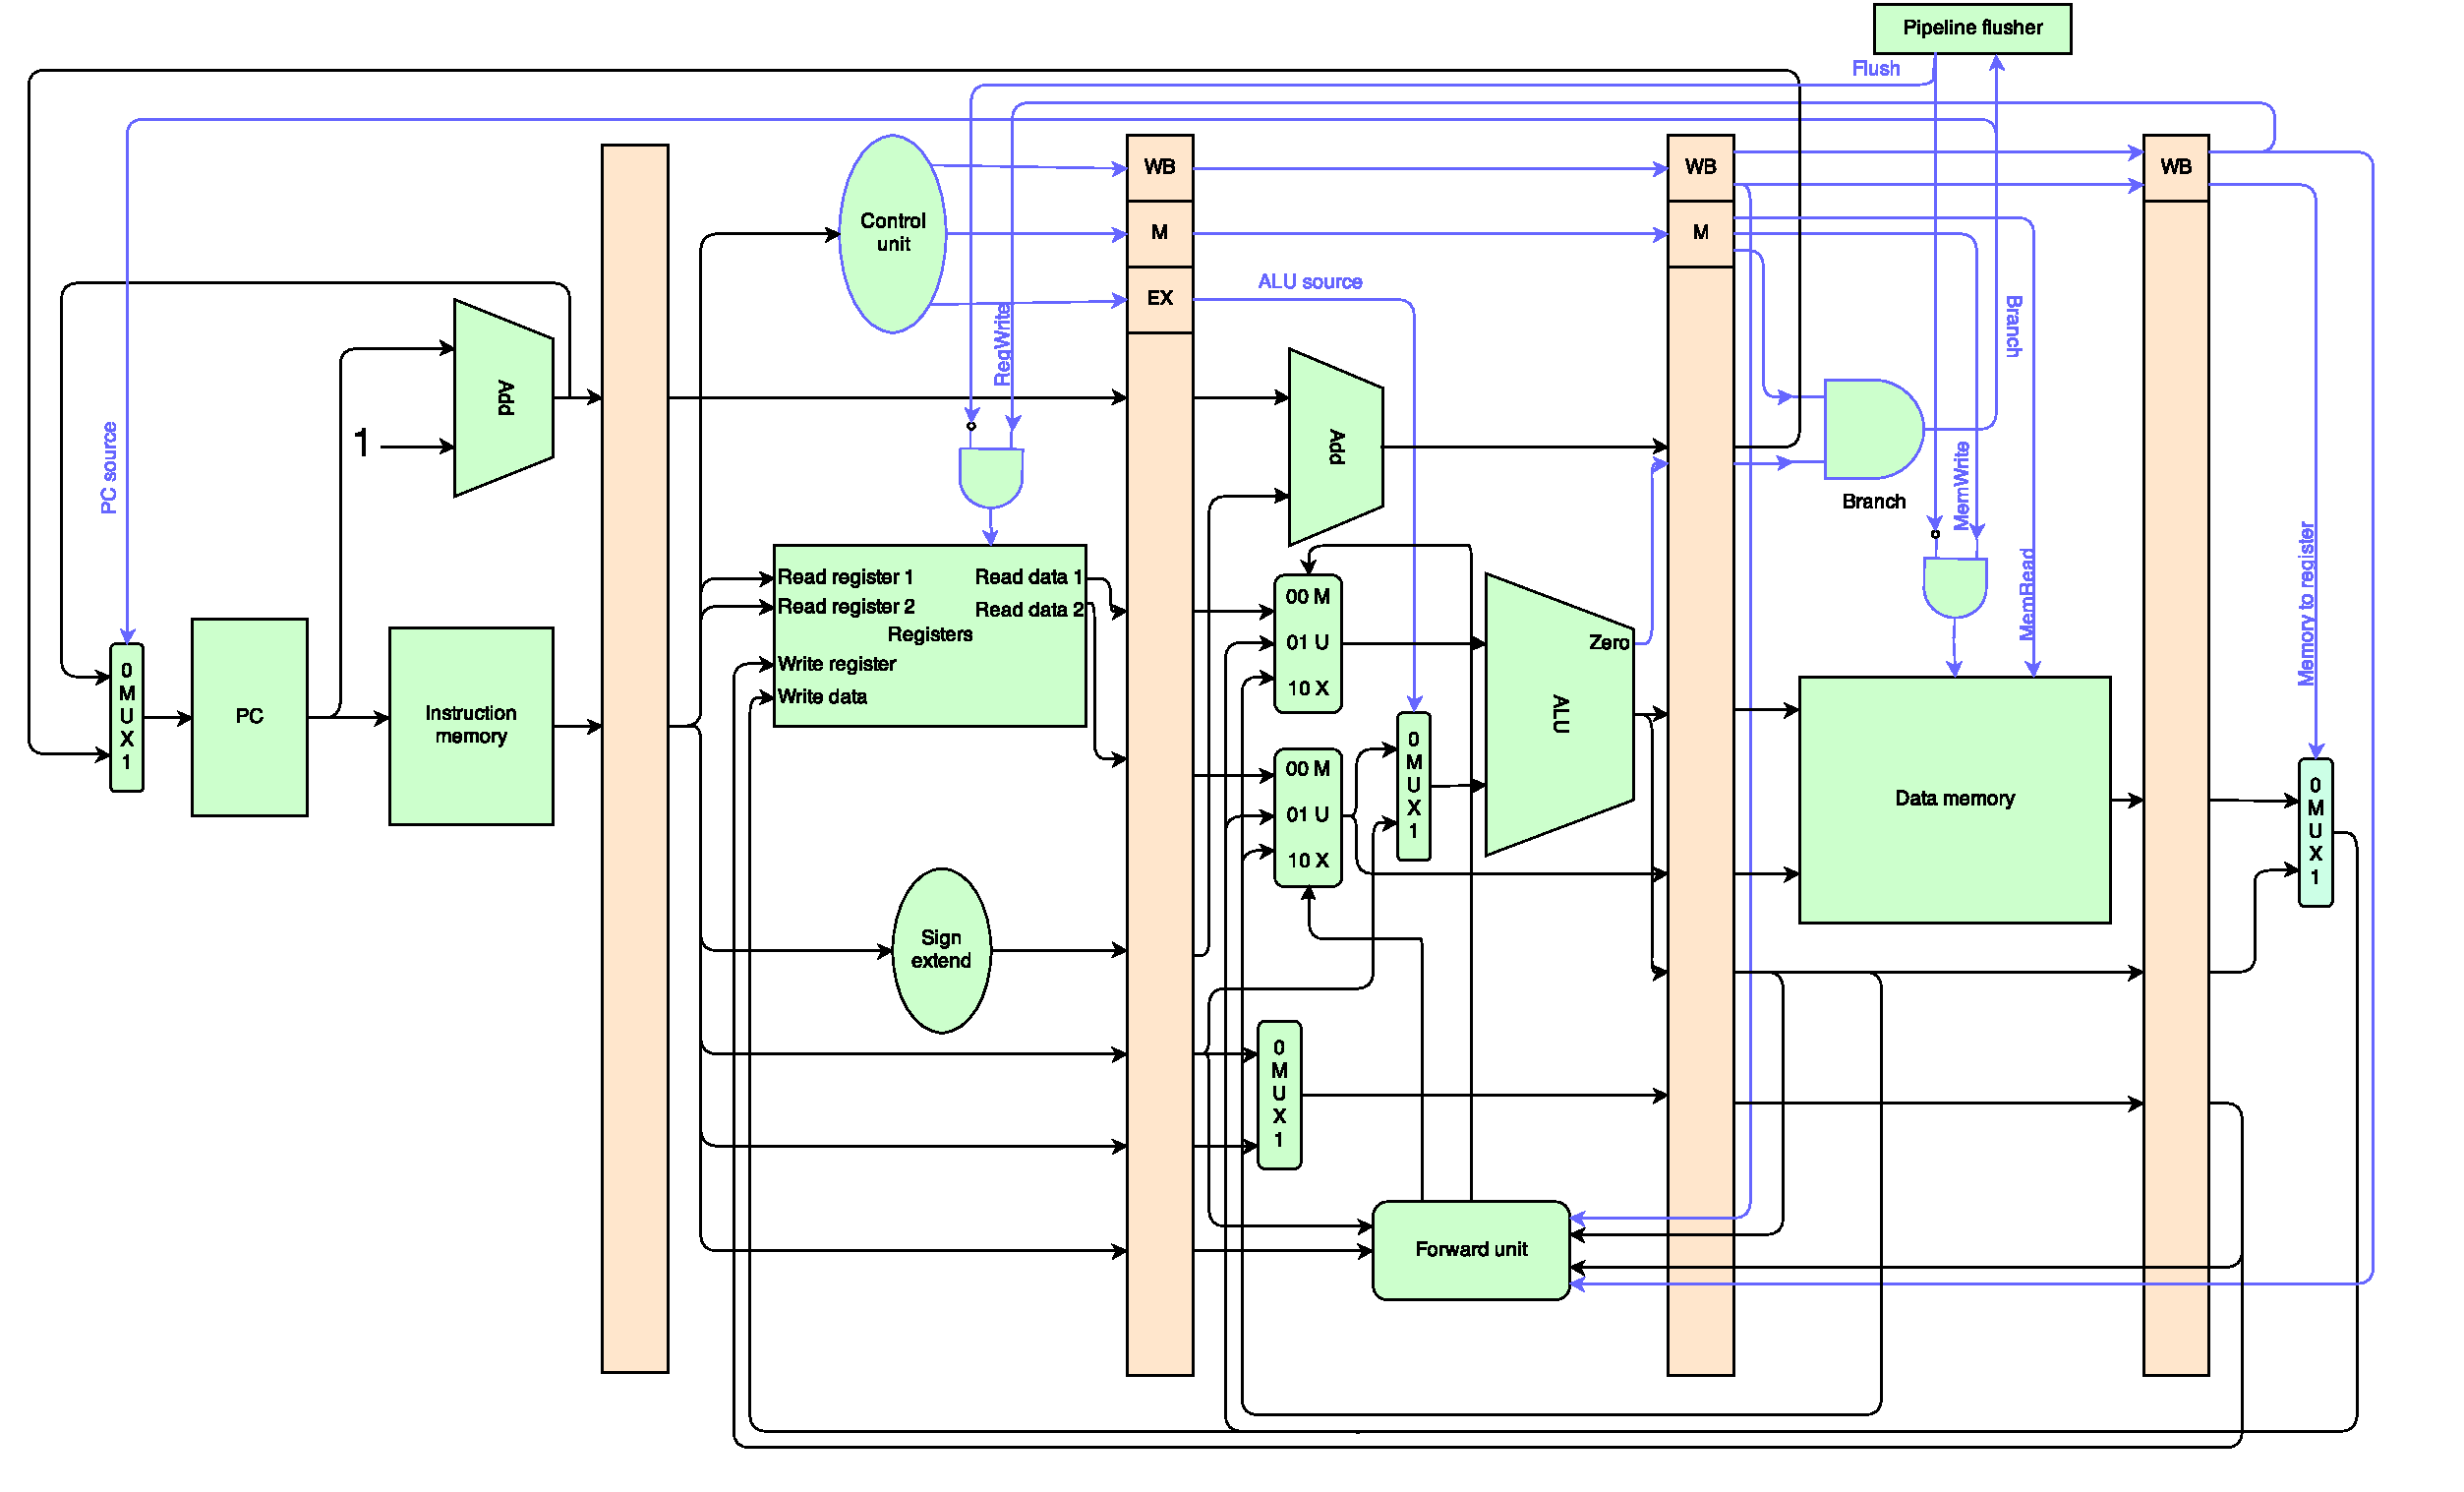
\includegraphics[width=\textwidth]{illustrations/processor.pdf}
    \caption{The processor architecture}
    \label{figure:architecture}
\end{figure}


The rest of this section describes the different architectural sub-components in detail.

\subsection{Instruction Fetch Stage}
    The instruction fetch stage is the first stage in the processor pipeline.
It is responsible for fetching the correct instruction from the instruction memory, and feeding it to the next stage in the pipeline.

\subsubsection{Program Counter}
In order to know where in the program the processor is currently executing, a program counter is needed.
The program counter is a simple register which holds the instruction address of the address currently being fetched and sent on to the next stage in the pipeline.
The instruction fetch stage updates the program counter each cycle, either by increasing it by one so as to fetch the next instruction, or by to a different number requested by a different part of the processor, in the case of a jump.



\subsection{Instruction Decode Stage}
    \todo{picture of decode stage}

The instruction decode stage receives an instruction from the instruction fetch stage and understands it.
Using this understanding, it orchestrates and coordinates the execution of the instruction.
This means that it is responsible for preparing the necessary data for the ALU, and setting the appropriate control signals for the rest of the processor for each instruction.
The register file of the processor resides in the instruction decode stage, and register data that are needed in computation in the execution stage are fetched and prepared in the instruction decode stage.
The control unit also resides in this stage.

\newpage
\subsubsection{Register File}
    \input{solution/solution-architecture/id-stage/register-file.tex}

\newpage
\subsubsection{Control Unit}
    \input{solution/solution-architecture/id-stage/control-unit.tex}


\subsection{Execution Stage}
    \todo{describe this stage}
\todo{image of this stage}

\subsubsection{ALU}
    \input{solution/solution-architecture/ex-stage/alu.tex}

\subsubsection{Forwarding Unit}
    \input{solution/solution-architecture/ex-stage/forwarding-unit.tex}

\subsubsection{Hazard Detector}
    \input{solution/solution-architecture/ex-stage/hazard-detector.tex}


\subsection{Memory Stage}
    \subsubsection{Data Memory}


\subsection{Write-Back Stage}
    The Write Back stage is responsible for routing the correct data to the register file, when data should be written to the register file.


\subsection{Additional Components}
    \subsubsection{Pipeline Registers}

Between each stage of the pipeline there are series of registers that hold the necessary values between clock ticks.
The pipeline registers are clocked synchronously, which means that the pipeline design is a buffered synchronous design.
The pipeline registers are implemented as flip-flops.


\subsubsection{Flip Flop}

A flip-flop is a simple circuit that has two stable states.
The implication is that they can be used to store values over time.

In the solution processor, size-generic flip-flops VHDL are used.
Because type generics were first introduced in the VHDL 2008 standard\cite{vhdl2008}, and the Xilinx tool chain doesn't support it yet, flip-flops are implemented on a per-type basis.
Subsequently, the \texttt{flip\_flop.vhd} VHDL source code file is a lot bigger and hairier than it could be.

\subsubsection{Multiplexers}

A multiplexer is a component which selects between multiple input signals based on a separate control signal.
Since multiplexers are use quite commonly, and VHDL has no build in construct for it, some multiplexer components are introduced in the solution.

\subsubsubsection{Multiplexer 2}

The Multiplexer 2 selects one of two possible input values based on the value of a 1-bit selection signal.

\subsubsubsection{Multiplexer 3}

The Multiplexer 3 selects one of three possible input values based on the value of a 2-bit selection signal.
Since a 2-bit selection signal may have 4 possible states, and the Multiplexer 3 only has three inputs, one of the selection signal states ("\texttt{11}") holds undefined behaviour.

\subsubsection{Pipeline flusher}

The pipeline flusher is reponsible for flushing the pipeline if a branch prediction goes wrong.
In such a case, the pipeline will be filled with instructions that shouldn't be executed.
The pipeline flusher disables these instructions by removing their ability to write to registers and memory.



\subsection{ALU}

The ALU in the solution processor has been completely rewritten from scratch.
This was done so that the IEEE industry standard packages \texttt{numeric\_std} could be used.
Using \texttt{numeric\_std}, developers can safely express complex processes in a succinct and easy-to-read fashion, using the many built-in features.
Using industry standards for the solution processor was a goal for two reasons.
First, choosing the conventions and standards recommended by the industry is typically a good idea, as industry leaders have a lot of experience in their field.
Second, using well-documented and feature-rich standard libraries facilitate the implementation of many different CPU instructions, which was a prioritized goal for this exercise.

Although the suggested architecture in the compendium features an ALU control unit\cite{compendium}, it does not exist in the solution architecture.
Instead, the ALU control unit's responsibilities are covered for by the regular control unit.
This design choice was made for the flexibility it provides in implementing more instructions.

\subsection{Branch Controller}

The branch controller the logic unit that decides whether or not the program should branch.
It is separate from the main control unit, as it works independently from the control unit state machine, and does not need to follow the clock.
The branch controller reads the opcode field from the current instruction, looking for branch instructions.
If it finds a branch instruction, it will apply the logic that is required for that instruction.

Having branch logic contained in a separate branch controller gives the opportunity to implement many different branch instructions in a modular manner.

To handle the simplest operations that compare two registers to each other, the branch controller can simply look at the flags from the ALU to decide if the branch MUX should be enabled.
Instructions that compare a register to zero require a bit more work from the branch controller.
The branch controller can send out a zero value that overrides the ALU's source for the $ y $ operand, and is compared to the $ x $ operand from the register specified in the instruction.

To allow for other compare operations than $x \geq 0$ and $x < 0$, the zero value will not always be zero. 
Because the solution processor only handles integers, the comparison $ x \geq 1 $ is equivalent with $ x > 0 $.
This trick means that support for branch operations other than zero and negative are not needed, which nicely reduces complexity in the design without sacrificing performance.
Therefore the zero value from the branch controller vary from -1 to 1.

The control unit drives the branch controller by instructing the ALU to do a subtraction on its inputs, $ x - y $, and ignore the result.
This sets the zero flag of the ALU if the x = y, and the negative flag of the ALU if the x < y.
It is these flags that is used by the branch controller to detemin if it should branch.

\subsection{Control Unit}

The control unit is a finite state machine that controls the processor.
Its job is to maintain the control state across cycles, and distribute the correct control signals to the other components in the processor at the right time.
The finite state machine has three states: fetch, execute and stall.
It advances to the next state on every cycle, with transitions as illustrated in figure \ref{figure:control-unit-state-machine}.

\begin{figure}[h]
    \begin{center}
        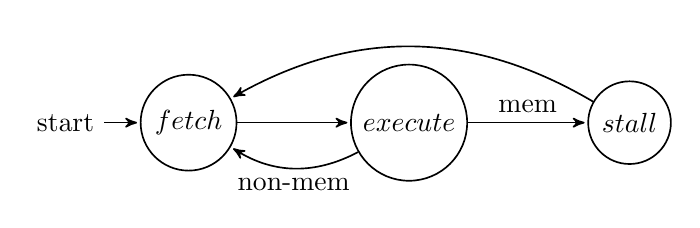
\begin{tikzpicture}[->,>=stealth',shorten >=1pt,auto,node distance=2.8cm, semithick]
            \tikzstyle{every state}=[fill=none,draw=black,text=black]
            \node[initial,state] (fetch)                    {$fetch$};
            \node[state]         (execute) [right of=fetch] {$execute$};
            \node[state]         (stall) [right of=execute] {$stall$};
            \path (fetch) edge node {} (execute)
                (execute) edge [bend left] node {non-mem} (fetch)
                (execute) edge node {mem} (stall)
                (stall) edge [bend right] node {} (fetch);
        \end{tikzpicture}
            \caption{
                Control unit state machine.
                \texttt{mem} transitions are taken when the currently executed instruction accesses memory.
            }
            \label{figure:control-unit-state-machine}
    \end{center}
\end{figure}

TODO: explain the signals that come out of the control unit

Here is a list for now populated by the signal names and Odd's educated guesses and brief explanations of the obvious.

\subsubsection{ALU Source}
The control signal for the ALU Source MUX. If 1 then the MUX selects the output from Sign Extend, if 0 it selects the signal from Read Data 2 in the Registers block.

\subsubsection{Register Write}
Does this turn on if we are writing to a register?

\subsubsection{Register Destination}
If 1 then the the Register Destination MUX outputs bits 15-11 of the instruction. If 0 then it outputs bits 20-16 of the instruction. Either way it feeds this to the Write Register port on the Registers block.

\subsubsection{Memory to Register}
Is this like, fetch? Are we putting memory in the registers?

\subsubsection{Memory Write}
I guess this is set if the instruction writes to memory?

\subsubsection{Jump}
The Jump signal indicates whether or not the current instruction is a jump instruction. If it is, the Jump signal is set to $1$ which causes the Jump MUX to output the Jump Address signal from Concat.

\subsection{Program Counter Cycle}

The program counter cycle is the loop the program counter forms together with the branch and jump circuitry.
The program counter is a D-latch register (TODO: is it?) that holds the address of the next instruction to be fetched.
When no branching or jumping is involved (the ``sunny day scenario''), the program counter cycle increments the program counter by one every cycle the control unit tells it to.
This means that the control unit has the opportunity to advance the running program.
The control unit advances the program counter when it is in the execute state, so that a new program counter value is ready for when the control unit enters the fetch state.

When the control unit gives the signal, the program counter may perform a branch or a jump by manipulating the program counter cycle to change the value sent back to the program counter.

TODO: diagram of the program counter cycle.

\subsection{Multiplexer}

The multiplexer... do we even need to talk about it?

\section{Instruction Set}

The solution processor implements a modified subset of the MIPS instruction set.
A quick reference of the MIPS instruction set can be found in Figure 3.4 of the compendium \cite{compendium}.
The instructions, as in regular MIPS, can be on one of three general formats, R, I and J.

The solution processor implements the instructions in table \ref{table:implemented-instructions}.
The processor supports quite a few more instructions than the minimum requirements.
This is done because (TODO: convincing argument).

\begin{table}
    \begin{center}
        \begin{tabular}{r|l}
            \texttt{ADD} & Add \\
            \texttt{ADDI} & Add immediate \\
            \texttt{ADDIU} & Add immediate unsigned \\
            \texttt{ADDU} & Add unsigned \\
            \texttt{AND} & And \\
            \texttt{ANDI} & And immediate \\
            \texttt{BEQ} & Branch if equal \\
            \texttt{BNE} & Branch not equal \\
            \texttt{J} & Jump \\
            \texttt{LUI} & Load upper immediate \\
            \texttt{LW} & Load word \\
            \texttt{MULT} & Multiply \\
            \texttt{MULTU} & Multiply unsigned \\
            \texttt{NOR} & Nor \\
            \texttt{OR} & Or \\
            \texttt{ORI} & Or immediate \\
            \texttt{PASSTHROUGH} & Passthrough (i.e. send the first input through unmodified) \\
            \texttt{SLL} & Shift left logical \\
            \texttt{SLLV} & Shift left logical variable \\
            \texttt{SLT} & Set less than \\
            \texttt{SLTI} & Set less than immediate \\
            \texttt{SLTIU} & Set less than immediate unsigned \\
            \texttt{SLTU} & Set less than unsigned \\
            \texttt{SRA} & Shift right arithmetic \\
            \texttt{SRAV} & Shift right arithmetic variable \\
            \texttt{SRL} & Shift right logical \\
            \texttt{SRLV} & Shift right logical variable \\
            \texttt{SUB} & Subtract \\
            \texttt{SUBU} & Subtract unsigned \\
            \texttt{SW} & Store word \\
            \texttt{XOR} & Xor \\
            \texttt{XORI} & Xor immediate \\
        \end{tabular}
        \smallskip
        \hrule
        \smallskip
        \caption{Implemented instructions}
        \label{table:implemented-instructions}
    \end{center}
\end{table}

\section{Test utilities}

TODO: move the solution component description of the test utilities from results-and-tests here

\section{Deliverables}

This is where we list all the deliverables we're sending in.


\chapter{Setup \& Tools}
	\section{Project Setup}

The Xilinx ISE project was set up with the design properties as in table \vref{table:design-properties}.

\begin{table}
    \begin{center}
        \begin{tabular}{ | l | l | }
            \multicolumn{1}{ l }{\textbf{Property Name}} &
            \multicolumn{1}{ l }{\textbf{Value}} \\
            \multicolumn{2}{ l }{ } \\
            \hline
            Top-Level Source Type & HDL \\
            \hline
            Family & Spartan6 \\
            Device & XC6SLX16 \\
            Package & CSG324 \\
            Speed & -3 \\
            \hline
            Synthesis tool & XST (VHDL/Verilog) \\
            Simulator & ISim (VHDL/Verilog) \\
            Preferred Language & VHDL \\
            Property Specification in Project File & Store non-default values only \\
            Manual Compile Order & (not checked) \\
            VHDL Source Analysis Standard & VHDL-93 \\
            \hline
            Enable Message Filtering & (unchecked) \\
            \hline
        \end{tabular}
        \caption{Xilinx ISE Project Design Properties}
        \label{table:design-properties}
    \end{center}
\end{table}

\todo{Verify that this table is still correct}

\section{Tools}

This section contains a description list of the tools used for the assignment.

\todo{Add any more stuff here}

\subsection{Software}
\begin{description}
    \item{\textbf{ISE Project Navigator 12.4 (nt64) M.81d, expired licence}} \\
        Main IDE for writing VHDL.
    \item{\textbf{ISim 12.4 (nt64) M.81d, expired license}} \\
        Main simulation environment for simulating VHDL.
    \item{\textbf{ModelSim SE 6.6d}} \\
        Secondary simulation environment for simulating VHDL.
    \item{\textbf{Xilinx Platform Studio 12.4 (nt64) Build EDK\_MS4.81d+1, expired licence}} \\
        Used for preparing compiled VHDL for the FPGA board.
    \item{\textbf{Avnet Programming Utility}} \\
        Used for configuring the FPGA.
    \item{\textbf{Text editors}} \\
        Sublime Text 2, Vim 7.3, Notepad (©Copyright Microsoft Corporation).
    \item{\textbf{GHDL 0.29 (2010109) [Sokcho edition]}} \\

    \item{\textbf{GNU command-line tools}} \\
        Grep, sed, find, etc.
    \item{\textbf{git 1.8.1.2}} \\
        Version control system.
    \item{\textbf{GitHub}} \\
        Remote code repository hosting, issue tracking, wiki for logging.
\end{description}

\subsection{Hardware}
\begin{description}
\item{\textbf{Xilinx Spartan-6 XC6SLX16 CSG324}}
    FPGA board.
\item{\textbf{Development PC, Windows 7}}
    For development.
\item{\textbf{Mini USB cable}}
    For connecting the FPGA board to the development computer.
\end{description}


\subsection{Linux Tool Chain}

In addition to the Windows-based proprietary Xilinx tool chain available in the lab\cn, a Linux-based free open source tool called GHDL was used.
GHDL is the leading open source VHDL compiler\cn, and offers many benefits over the clunky Xilinx tool chain for rapid development and iteration.
Although it is not as feature-rich as the Xilinx tools, and does not offer critical functionality such as synthesizing, it out-performs Xilinx in other areas.
Two areas in which it excels are intelligent error messages during analysis, and speed of compilation.
As a comparison, consider a typical error message from Xilinx ISE in figure \vref{figure:xilinx-error-message}, and compare it to the error message produced by GHDL for the same error in \vref{figure:ghdl-error-message}.
This error was produced by removing the keyword \texttt{begin} from the architecture begin statement of the \texttt{flip\_flip} entity.
Especially dumbfounding is the error message in figure \vref{figure:xilinx-error-message} referring to an \texttt{is\_x}.
At no point in the VHDL code is there any string even remotely resembling \texttt{is\_x}.
The GHDL error message in figure \vref{figure:ghdl-error-message}, on the other hand, is short and concise, and actually tells the programmer exactly what is wrong, and what can be done to fix it.

\begin{figure}
\texttt{
flip\_flop.vhd:17:5: object class keyword such as 'variable' is expected
flip\_flop.vhd:21:9: 'begin' is expected instead of 'elsif'
}
\begin{center}
\caption{A typical error message from GHDL.}
\label{figure:ghdl-error-message}
\end{center}
\end{figure}

\begin{figure}
\texttt{
Line 27: Syntax error near "flip\_flop".\\
Line 27: Expecting type  void for <flip\_flop>.\\
Line 29: Syntax error near "behavioral".\\
Line 29: Expecting type  void for <behavioral>.\\
Line 32: Expecting type  void for <ieee>.\\
Line 33: is\_x is not a  void\\
Line 33: Formal <s> has no actual or default value.\\
s is declared here\\
Line 35: Syntax error near "entity".\\
...\\
}
\begin{center}
\caption{A typical error message from Xilinx ISE.}
\label{figure:xilinx-error-message}
\end{center}
\end{figure}


\chapter{Results and Tests}
	\section{VHDL Test Benches}

In VHDL, one has the opportinity to create test benches to validate VHDL components.
A test bench is a piece of VHDL code that instantiates a component, manipulates its in-signals, and measures the output the component sends out again.
It is the hardware design analog of unit testing in regular software development.
These test benches are typically run in simulator software such as ISim or ModelSim, which simulates hardware in an easily measurable and inspectable environment.

Generally, each component made in VHDL should have a corresponding test bench.
Because a component is typically defined in its own file, a common test bench scheme is to have one file, ``\texttt{my\_entity.vhd}'', which defined the component, and one file, ``\texttt{tb\_my\_entity.vhd}'', which defines the test bench for the component.
Of course, here \texttt{my\_component} is a placeholder name for a component.

In this assignment, each component has an corresponding automatic test bench, which aims to verify correct functionality for a component.
The tests were run in the hardware simulation tool called ISim 12.4 (nt64).
See appendix (TODO: appendix numbers) for detailed results of each test bench simulation.

\subsection{ALU Test Bench}

The alu is continously receiving values for x, y and func, and will use this input to set the correct values for r and the flags.
The test bench include tests for the outputs for each of the alus supported functions.
In addition the subtraction function is tested extra thuraly.
This is because of it's involvement in the branch operations.

\subsection{Branch Controller Test Bench}

The branch controller is a logical unit that will continuously determin if the alu should compare to a zero value, and whether or not to branch.
The test will check each branching operation and test that the compare\_zero and compare_\zero\_value have the correct values.
The test will also check each of these operations with their sensitive flag on and off, and test that branch have the right value.
For good measure we also check that all values is set to 0 when the operation is not a branching operation.
This last test is not really nesseccary in the current processor layout as the branching mux will remove the signal eventually.

\subsection{MUX Test Bench}

The MUX is really quite simple, and so is its test.
The test put two different signals on the input ports and read each of these through each of the imput ports.

\subsection{Pc Test Bench}

The program counter have several inputs which on each rising edge on the clock will reevaluate what value to put out of the program counter.
There are several ways the programcounter can act:
* If reset is set to 1, it will reset pc\_out to 0.
* If both pc enable and reset is set to 1, it should still reset.
* If pc enable is set to 0, it will not load a new value from pc\_in.
* If pc enable is set to 1, pc\_out will be set to the value of pc\_in.
We test that each of these 4 behaviors work as intended.


\subsection{Processor Test Bench}

The processor test bench test that the processor act as expected on a few operations.
First it load some numbers into registers.
When these data are ready, the test do some math on the data.
In the end the data is writen back to memory.
The purpose of this test is not to cover all the operations, as they are already covered in the alu test bench.
The processor test bench will make sure that all of the processors components are working together, and that it is able to execute memory load and store operations.

\subsection{Toplevel Test Bench}

The toplevel test bench defines a short program of 16 binary-coded instructions that it uses to test the processor.
These instructions are helpfully named \texttt{ins0} through \texttt{ins15}.
A comment in the the test bench refers to a certain \texttt{ins.txt}, which supposedly contains a description of the instructions, but it is nowhere to be found.
A manually decoded program listing of this program can be found in listing \vref{listing:toplevel-program}.

\begin{listing}
\begin{center}
\begin{bytefield}[rightcurly=., rightcurlyspace=0pt, leftcurly=., leftcurlyspace=0pt]{32}
\bitheader[endianness=big]{0-16,20,21,25,26,31} \\

\begin{rightwordgroup}{\texttt{lw r0, 1(r0)}}
\begin{leftwordgroup}{\texttt{ins0}}
\bitbox{6}{op: lw \\ \tiny 100011}
& \bitbox{5}{rs: r0 \\ \tiny 00000}
& \bitbox{5}{rt: r1 \\ \tiny 00001}
& \bitbox{16}{immediate: 1 \\ \tiny 0000000000000001}
\end{leftwordgroup}
\end{rightwordgroup} \\

\begin{rightwordgroup}{\texttt{lw r2, 2(r0)}}
\begin{leftwordgroup}{\texttt{ins1}}
\bitbox{6}{op: lw \\ \tiny 100011}
& \bitbox{5}{rs: r0 \\ \tiny 00000}
& \bitbox{5}{rt: r2 \\ \tiny 00010}
& \bitbox{16}{immediate: 1 \\ \tiny 0000000000000010}
\end{leftwordgroup}
\end{rightwordgroup} \\

\begin{rightwordgroup}{\texttt{lw r2, 2(r0)}}
\begin{leftwordgroup}{\texttt{ins2}}
\bitbox{6}{op: lw \\ \tiny 100011}
& \bitbox{5}{rs: r0 \\ \tiny 00000}
& \bitbox{5}{rt: r2 \\ \tiny 00010}
& \bitbox{16}{immediate: 1 \\ \tiny 0000000000000010}
\end{leftwordgroup}
\end{rightwordgroup} \\

\begin{rightwordgroup}{\texttt{add r3, r1, r2}}
\begin{leftwordgroup}{\texttt{ins3}}
\bitbox{6}{op: r\_all \\ \tiny 000000}
& \bitbox{5}{rs: r1 \\ \tiny 00001}
& \bitbox{5}{rt: r2 \\ \tiny 00010}
& \bitbox{5}{rd: r3 \\ \tiny 00011}
& \bitbox{5}{sh: 0 \\ \tiny 00000}
& \bitbox{6}{func: add \\ \tiny 100000}
\end{leftwordgroup}
\end{rightwordgroup} \\

\begin{rightwordgroup}{\texttt{sw r3, 5(r0)}}
\begin{leftwordgroup}{\texttt{ins4}}
\bitbox{6}{op: sw \\ \tiny 101011}
& \bitbox{5}{rs: r0 \\ \tiny 00000}
& \bitbox{5}{rt: r3 \\ \tiny 00011}
& \bitbox{16}{imm: 5 \\ \tiny 0000000000000101}
\end{leftwordgroup}
\end{rightwordgroup} \\

\begin{rightwordgroup}{\texttt{beq r0, r0, 5}}
\begin{leftwordgroup}{\texttt{ins5}}
\bitbox{6}{op: beq \\ \tiny 000100}
& \bitbox{5}{rs: r0 \\ \tiny 00000}
& \bitbox{5}{rt: r0 \\ \tiny 00000}
& \bitbox{16}{imm: 5 \\ \tiny 0000000000000101}
\end{leftwordgroup}
\end{rightwordgroup} \\

\begin{rightwordgroup}{\texttt{sw r3, 3(r0)}}
\begin{leftwordgroup}{\texttt{ins6}}
\bitbox{6}{op: sw \\ \tiny 101011}
& \bitbox{5}{rs: r0 \\ \tiny 00000}
& \bitbox{5}{rt: r3 \\ \tiny 00011}
& \bitbox{16}{imm: 3 \\ \tiny 0000000000000011}
\end{leftwordgroup}
\end{rightwordgroup} \\

\begin{rightwordgroup}{\texttt{sw r3, 4(r0)}}
\begin{leftwordgroup}{\texttt{ins7}}
\bitbox{6}{op: sw \\ \tiny 101011}
& \bitbox{5}{rs: r0 \\ \tiny 00000}
& \bitbox{5}{rt: r3 \\ \tiny 00011}
& \bitbox{16}{imm: 4 \\ \tiny 0000000000000100}
\end{leftwordgroup}
\end{rightwordgroup} \\

\begin{rightwordgroup}{\texttt{sw r3, 6(r0)}}
\begin{leftwordgroup}{\texttt{ins8}}
\bitbox{6}{op: sw \\ \tiny 101011}
& \bitbox{5}{rs: r0 \\ \tiny 00000}
& \bitbox{5}{rt: r3 \\ \tiny 00011}
& \bitbox{16}{imm: 6 \\ \tiny 0000000000000110}
\end{leftwordgroup}
\end{rightwordgroup} \\

\begin{rightwordgroup}{\texttt{sw r3, 7(r0)}}
\begin{leftwordgroup}{\texttt{ins9}}
\bitbox{6}{op: sw \\ \tiny 101011}
& \bitbox{5}{rs: r0 \\ \tiny 00000}
& \bitbox{5}{rt: r3 \\ \tiny 00011}
& \bitbox{16}{imm: 7 \\ \tiny 0000000000000111}
\end{leftwordgroup}
\end{rightwordgroup} \\

\begin{rightwordgroup}{\texttt{lui r3, 6(r0)}}
\begin{leftwordgroup}{\texttt{ins10}}
\bitbox{6}{op: lui \\ \tiny 001111}
& \bitbox{5}{rs: r0 \\ \tiny 00000}
& \bitbox{5}{rt: r3 \\ \tiny 00011}
& \bitbox{16}{imm: 6 \\ \tiny 0000000000000110}
\end{leftwordgroup}
\end{rightwordgroup} \\

\begin{rightwordgroup}{\texttt{sw r3, 8(r0)}}
\begin{leftwordgroup}{\texttt{ins11}}
\bitbox{6}{op: sw \\ \tiny 101011}
& \bitbox{5}{rs: r0 \\ \tiny 00000}
& \bitbox{5}{rt: r3 \\ \tiny 00011}
& \bitbox{16}{imm: 8 \\ \tiny 0000000000001000}
\end{leftwordgroup}
\end{rightwordgroup} \\

\begin{rightwordgroup}{\texttt{add r1, r3, r3}}
\begin{leftwordgroup}{\texttt{ins12}}
\bitbox{6}{op: r\_all \\ \tiny 000000}
& \bitbox{5}{rs: r1 \\ \tiny 00001}
& \bitbox{5}{rt: r3 \\ \tiny 00011}
& \bitbox{5}{rd: r3 \\ \tiny 00011}
& \bitbox{5}{sh: 0 \\ \tiny 00000}
& \bitbox{6}{func: add \\ \tiny 100000}
\end{leftwordgroup}
\end{rightwordgroup} \\

\begin{rightwordgroup}{\texttt{sw r3, 9(r0)}}
\begin{leftwordgroup}{\texttt{ins13}}
\bitbox{6}{op: sw \\ \tiny 101011}
& \bitbox{5}{rs: r0 \\ \tiny 00000}
& \bitbox{5}{rt: r3 \\ \tiny 00011}
& \bitbox{16}{imm: 9 \\ \tiny 0000000000001001}
\end{leftwordgroup}
\end{rightwordgroup} \\

\begin{rightwordgroup}{\texttt{beq r0, r0, -3}}
\begin{leftwordgroup}{\texttt{ins14}}
\bitbox{6}{op: beq \\ \tiny 000100}
& \bitbox{5}{rs: r0 \\ \tiny 00000}
& \bitbox{5}{rt: r0 \\ \tiny 00000}
& \bitbox{16}{imm: -3 \\ \tiny 1111111111111101}
\end{leftwordgroup}
\end{rightwordgroup} \\

\begin{rightwordgroup}{\texttt{sw r3, 10(r0)}}
\begin{leftwordgroup}{\texttt{ins15}}
\bitbox{6}{op: sw \\ \tiny 101011}
& \bitbox{5}{rs: r0 \\ \tiny 00000}
& \bitbox{5}{rt: r3 \\ \tiny 00011}
& \bitbox{16}{imm: 10 \\ \tiny 0000000000001010}
\end{leftwordgroup}
\end{rightwordgroup} \\

\end{bytefield}
\end{center}
\caption{The short program in the toplevel test bench}
\label{listing:toplevel-program}
\end{listing}


\section{Testing on the Spartan-6 FPGA}

It is also possible to run toplevel test benches directly on the FPGA (I think).
TODO: write more about this.

\section{Physical Measurements}

TODO: insert energy efficiency measurements, or something.

This is what the results of such tests may have looked like:
Audible noise test: low audibility. (there are no moving parts)

Energy consumption test:
upper bound: <upper bound of the FPGA>
lower bound: >1 




\chapter{Discussion}
	Discuss the assignment and your achievements.
You are free to critically assess your work:
what could have been done better, which way you would choose to go if given the same task again etc.

This chapter discusses the performance and test results of the presented solution processor, as well as the assignment it self and the work process around it.

\section{Industry Standard Best Practices}

Did we meed the goal about conforming to industry standards?
What are the industry standards?

VHDL is a language defined by standards laid forth by IEEE, the Institute of Electrical and Electronics Engineers.
In order to write good VHDL, it is best to use IEEE-sanctioned standard libraries.

\subsection{\texttt{numeric\_std}}


For doing arithmetic operations on logic vectors in VHDL, many resources (TODO: cite! websites, tutorials, books) will suggest using the functionality provided in the packages \texttt{ieee.std\_logic\_arith} and \texttt{ieee.std\_logic\_unsigned}.
These packages are non-standard packages defined by a company called Synposis, which makes one of the more popular VHDL tool suites.
Synopsis bundles these packages in their tool distributions, which causes a lot of confusion as to whether or not a part of the standard VHDL library.
Unfortunately, because of this, these non-standard packages have enjoyed wide-spread usage amongst VHDL coders.
This is a problem, because different vendors of VHDL tools have begun supply their own versions of \texttt{std\_logic\_arith} and \texttt{std\_logic\_unsigned}.
Of course, as there is no standard governing these packages, the different versions supplied by different versions have begun to diverge, and are not necessarily compatible with each other.

IEEE has countered this problem by defining new standard packages called \texttt{numeric\_std} and \texttt{numeric\_bit}, which implement similar functionality as the unofficial Synposis packages.
This ensures compatibility across VHDL tools from different vendors.

\texttt{Numeric\_std} has a number of advantages over \texttt{std\_logic\_arith}.
The biggest advantage is that it defines new types for arithmetical logcal vectors, \texttt{signed} and \texttt{unsigned}, as opposed to trying to use \texttt{std\_logic\_vector} directly, which is what the Synopsis packages do.
This is an advantage because combining signed and unsigned arithmetic on the same signals becomes a lot easier.
In fact, the Synposis packages simply assumes all operands are unsigned in all arithmetic operations, which is a bad idea.
A different advantage with the standard packages is that they provide stronger quality assurance through type checking, as they introduce new types.
This is a good thing because it lets developers find bugs earlier, speeding up the development process.

In the solution VHDL code, all arithmetical operations are sanely implemented using \texttt{numeric\_std}.

TODO: citation to this thing might be a good idea: http://vhdlguru.blogspot.no/2010/03/why-library-numericstd-is-preferred.html .

\subsection{Test Coverage}

The solution processor has very good simulation test coverage.
Every custom entity in the solution VHDL code has its own extensive test bench, which uses the custom-made convenience functions from the \texttt{test\_utils} package.
Unfortunately, the solution processor was never tested physically on the FPGA, due to unfortunate prioritization in the design goals for the assignment.

To improve the test coverage, the obvious next step is to load the solution processor onto an FPGA and run the same tests on the physical board.

\subsection{Additional industry standards?}

TODO: Lets google some stuff and shoehorn it into this report.

\section{Instruction Set}

To what extent did we meet the design goal of having a large instruction set?
Was it a good idea to choose this as a design goal? (Hint: no).

\section{Performance}

The presented solution processor performs rather well for a sequential simple multi cycle processor.
The clock's maximum speed is (TODO: insert max clock speed).
In testing, it performs reliably in with clock speeds up to X at temperature Y.
Being a multi-cycle processor, most instructions take more than one cycle to complete.
Instructions that only operate on immediates and registers take two cycles to complete.
Instructions that access the data memory require an additional cycle, for a total of three cycles.
This means that under optimal conditions, the processor is capable of X/2 instructions per second (ref IPS).

One way of increasing performance beyond what has been done in the solution is to restructure the logical flow of the architecture to keep the data flow dependencies to a minimum.
Doing so would mean that the processor would need less time to stabilize for each cycle, and as an effect, the clock cycle speed could be increased.
As we all remember from Intel and AMD marketing in the early 2000's, more MHz means more power!

To further increase performance, we could introduce instruction-level parallelism in the form of a pipeline.
This, however, is out of the scope of this exercise.

\section{Energy Efficiency}

Any computer-related report worth its salt should ontain a section that discusses the energy efficiency of the presented solution.
This report is no different.
The solution processor was not designed with energy efficiency as a primary design goal.
It does, however strive for simplicity in its VHDL design, using official IEEE-reccomended industry standards for as many operations as possible.
This lets the synthesizer use its intimate knowledge of the feature set of the target FPGA to create customized hardware configurations that exploit the possibilities the FPGA provides.
This means that dedicated utility slices, block ram sections and similar will be used where possible.
They are typically faster than their custom logic counterparts, and therefore allow for quicker execution.
Although quicker execution by virtue of increased clock speeds does not change the energy efficiency of the processor for finite terminating programs, it may allow other dependant components in a larger system to enter low energy states quicker, and thereby reducing static energy loss in the system as a whole.

To make the processor more energy efficient, sleep states could be introduced.
They allow the processor to enter low energy states when it is not needed, i.e. typically when it is waiting for an external signal in a larger system, and when it has nothing else useful to do.

\section{About the Work Process}

TODO: bla bla, we should have started sooner, yadda yadda, could have done more etc, happy with final outcome.

also we could just go through our logs and see what we actually did and in what order.

THAT'S WHAT LOGS ARE FOR, YEAH.

TODO: attach an appendix of all the raw logs?


\chapter{Conclusion}
	The assignment was completed and the requirements were met.
Two additional design goals were set and prioritized by importance, which heavily influenced the solution.
The solution processor is capable of executing a comfortably large number of instructions in a performant manner, all the while following the recommended best practices put forth by IEEE and prominent VHDL gurus, as documented in \cite{assignment-1}.
The processor was successfully programmed onto the FPGA, but due to what was probably a fluke in the communication setup, data could not be read back from the running processor.

The assignment was surprisingly enough easier than than the previous assignment\cite{assignment-1}.
One reason for that is that the authors have become more proficient in VHDL and processor design in general, which has greatly helped speed up the design process.
A lot of the rookie mistakes that were made in \cite{assignment-1} were avoided in this assignment.
Additionally, for this assignment, a smaller implementation scope was wisely selected.

In conclusion, it was a fun assignment which was completed to reasonable satisfaction despite less than optimal time management within the group.



%% The bibliography should go here.

\bibliography{reference-library}{}
\bibliographystyle{plain}
\nocite{*} % renders the entire bibtex library in the bibliography, not just the entries that are cited


\end{document}
